% !TeX spellcheck = en_GB

\begin{figure}[htb]{0.5\textwidth}
	% Whole figure
	\begin{subfigure}[b]{\textwidth}
		% Start with figure wav
		\centering
		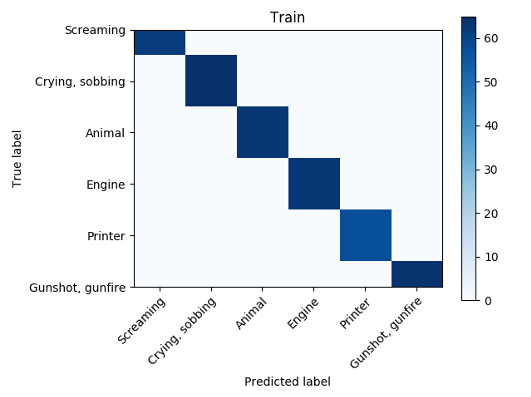
\includegraphics[width=0.4\linewidth]{wav_train}%
		\hfill
		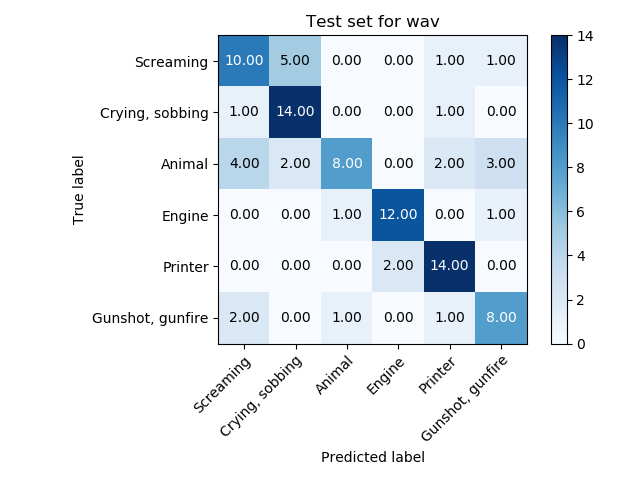
\includegraphics[width=0.4\linewidth]{wav_test}
		\subcaption{Confusion matrices when embeddings are extracted from audio files}
	\end{subfigure}
	\vskip\baselineskip
	% Start with figure tfrecord
	\begin{subfigure}[b]{\textwidth}
		\centering
		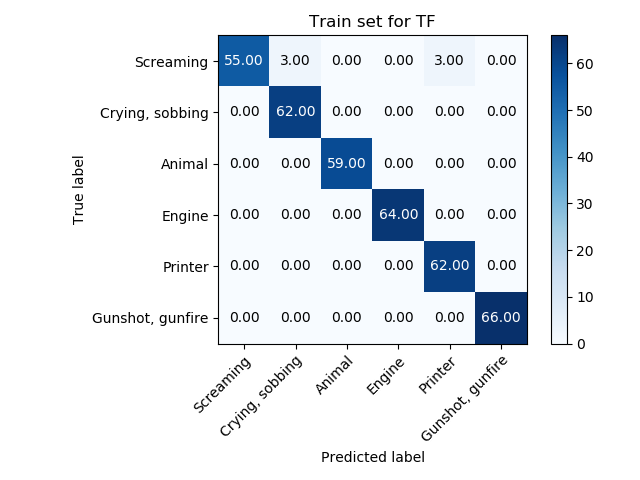
\includegraphics[width=0.4\linewidth]{tfrecord_train}%
		\hfill
		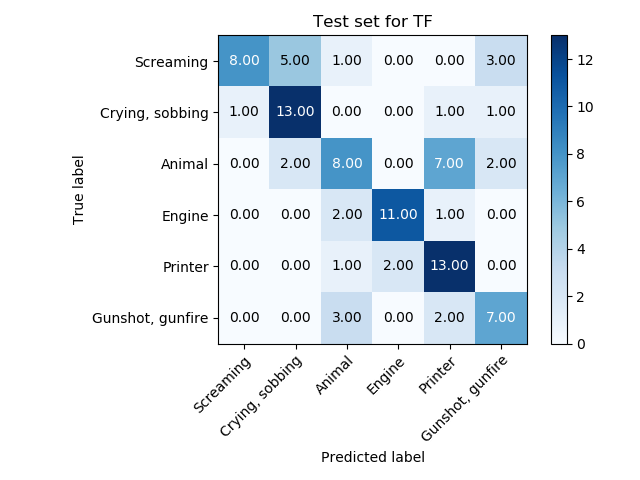
\includegraphics[width=0.4\linewidth]{tfrecord_test}
		\subcaption{Confusion matrices when embeddings are taken from .\textit{tfrecord} files}
	\end{subfigure}

	\caption{Confusion matrices}
	\label{fig:mesh7}
\end{figure}